\documentclass[11pt,a4paper]{article}
\usepackage[utf8]{inputenc}
\usepackage[T1]{fontenc}
\usepackage[slovene]{babel}
\usepackage{lmodern}
\usepackage{enumitem}
\usepackage{amsmath}
\usepackage{amssymb}
\usepackage{float} 
\usepackage{url} 
%\usepackage{hyperref} 
\usepackage{graphicx} 
\usepackage[margin=1.5cm]{geometry}
\usepackage{multirow}

\newcommand{\code}{\texttt}

\title{Vaje, vaje, vaje ... (DT)}
\author{Darja Turk}
\date{}

\begin{document}

\maketitle

\begin{enumerate}
    \item Natančno izračunaj $\displaystyle \tan\left(\frac{\pi}{4}-\alpha\right)$, če je $\displaystyle \sin\alpha=-\frac{5}{13}$ in $\pi<\alpha<\frac{3\pi}{2}$.
        \begin{flushright}
            $\left[\frac{7}{17}\right]$
        \end{flushright}

    \item Poenostavi izraz $\displaystyle \sin\left(x+\frac{5\pi}{2}\right)-\cos\left(2\pi-x\right)+\cos\left(x+\frac{3\pi}{2}\right)-\sin\left(x-\pi\right)$.
        \begin{flushright}
            $\left[2\sin x\right]$
        \end{flushright}

    \item Pokaži, da velja: $\displaystyle \frac{\cot x\cdot\sin{2x}-1}{\left(\cos(-x)-\sin(-x)\right)^2-1}=\cot{2x}$.

    \item Na sliki je graf funkcije $\displaystyle f(x)=A\sin\left(Bx+C\right)+D$. Določi $A>0$, $B>0$, $C$ in $D$. $C$~izberi tako, da bo $|C|$ najmanjše možno število. Kratko utemelji.
        \begin{figure}[H]
            \centering
            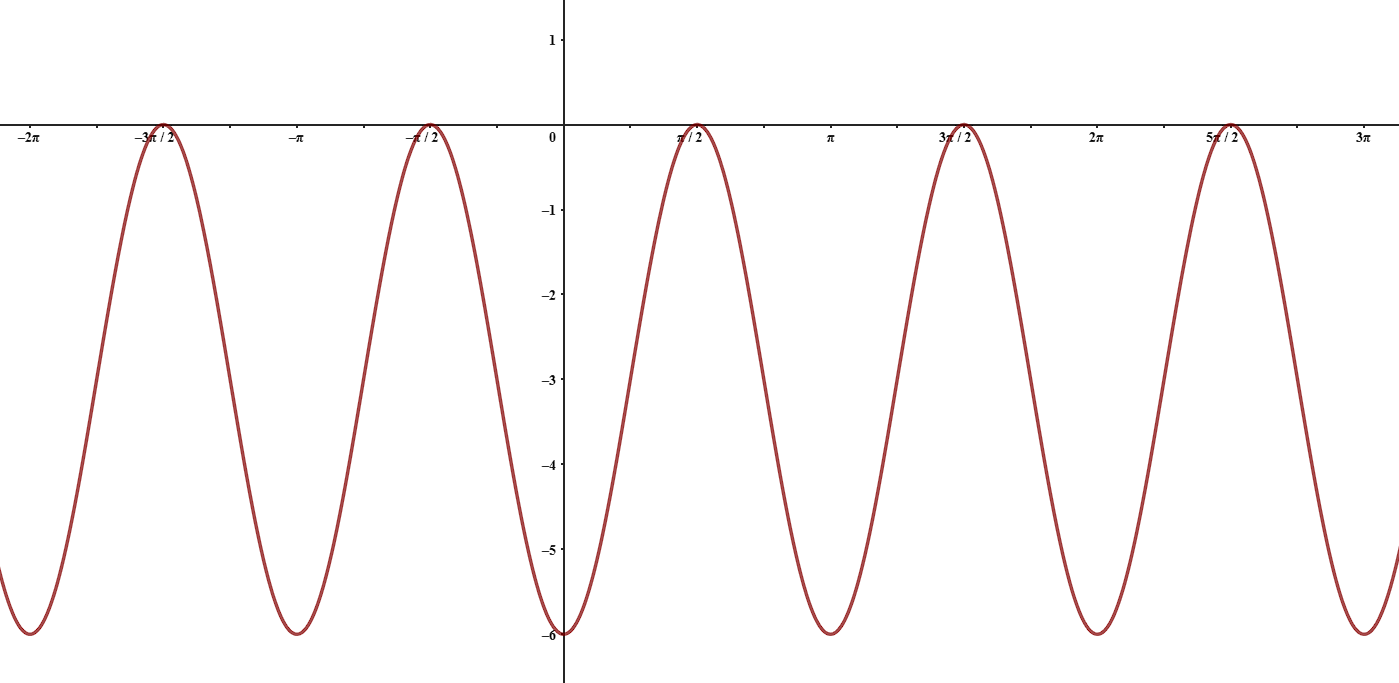
\includegraphics[scale=0.4]{../Slike in skice/vaje_vaje_vaje_sinus.png}
        \end{figure}
        \begin{flushright}
            $\left[f(x)=3\sin\left(2x-\frac{\pi}{2}\right)-3\right]$
        \end{flushright}


    \item Brez uporabe računala natančno izračunaj. Zapiši vmesne izračune.
        \begin{enumerate}
            \item $\displaystyle \sin\frac{23\pi}{6}$
            \item $\displaystyle \cos\left(-1590^\circ\right)$
        \end{enumerate}
        \begin{flushright}
            $\left[-\frac{1}{2};\ -\frac{\sqrt{3}}{2}\right]$
        \end{flushright}


    \item Reši enačbi:
        \begin{enumerate}
            \item $\displaystyle \sin{2x}+\sqrt{2}\cos x=0$
            \item $\displaystyle 2\cos^2{3x}-\cos{3x}-1=0$
        \end{enumerate}
        \begin{flushright}
            $\left[x\in \left\{\frac{\pi}{2}+k\pi;k\in\mathbb{Z}\right\}\cup\left\{-\frac{\pi}{4}+2k\pi;k\in\mathbb{Z}\right\}\cup\left\{\frac{5\pi}{4}+2k\pi;k\in\mathbb{Z}\right\} \right]$
            $\left[x\in \left\{k\frac{2\pi}{3};k\in\mathbb{Z}\right\}\cup\left\{\pm\frac{2\pi}{9}+\frac{2}{3}k\pi;k\in\mathbb{Z}\right\}\right]$
        \end{flushright}


\end{enumerate}


\end{document}